To start we design a small pilot study as a proof of concept with the aim to validate the classification and clustering methodology against the scale and complexity of data collected on a open public area such as a retail highstreet.
We also want to find the algorithm which is best suited for classification of signal strengths.
The data was collected at Oxford Street in London on 20 December 2017 from 12:30 to 13:00 hrs, where Wi-Fi probe requests sets were collected using the Wi-Fi sensor described earlier and pedestrian footfall was manually recorded using the Android app.
Being located at one of the busiest retail locations in the United Kingdom, the WiFi sensor captured approximately 60,000 probe requests during the period, and 3,722 people were recorded manually.

When we just aggregated the probe requests by their MAC address for every minute, the mean error between the sensor counts and the manual counts was observed to be on average 425\%.
This suggested that there was a large amount of noise in the data which might have included signals from devices outside the area where the manual count was conducted and anonymised probe requests with different MAC addresses from a few devices stationed next to the sensor.
We then classified the probe requests as "high signal strength" and "low signal strength" using `k-means' classification algorithm which resulted in the lowest mean error percentage closely followed by `quantile'.
The cut-off point or threshold for the collected data was -71 dBm.
We eliminated the noise from devices outside the area of interest by removing all the probe requests which reported a "low signal strength" below the threshold.
We found this process of filtering highly effective and reduced the mean minute by minute error to 30\%.

We then move on to assign an unique field identifying the mobile device generating the probe requests.
For the 45\% of the probe requests which were not randoised, we kept the MAC addresses as the unique identifier.
For the rest of the probe requesrt we applied the clustering alogorithm to assign the unique identifier.
With the help of the known stationary device (the mobile device used by the surveyor to record pedestrians manually) and through trail and error, We found the time threshold, $\alpha$ to be 15 seconds and threshold for sequence numbers, $\beta$ to be 60.
Figure \ref{pilot_clustering} shows the clustering of probe requests.
We finally combine both normal and anonymised probe requests, aggregate them based on their unique identifier which further reduced the mean error to -18\%.

\begin{figure}
	\begin{center}
		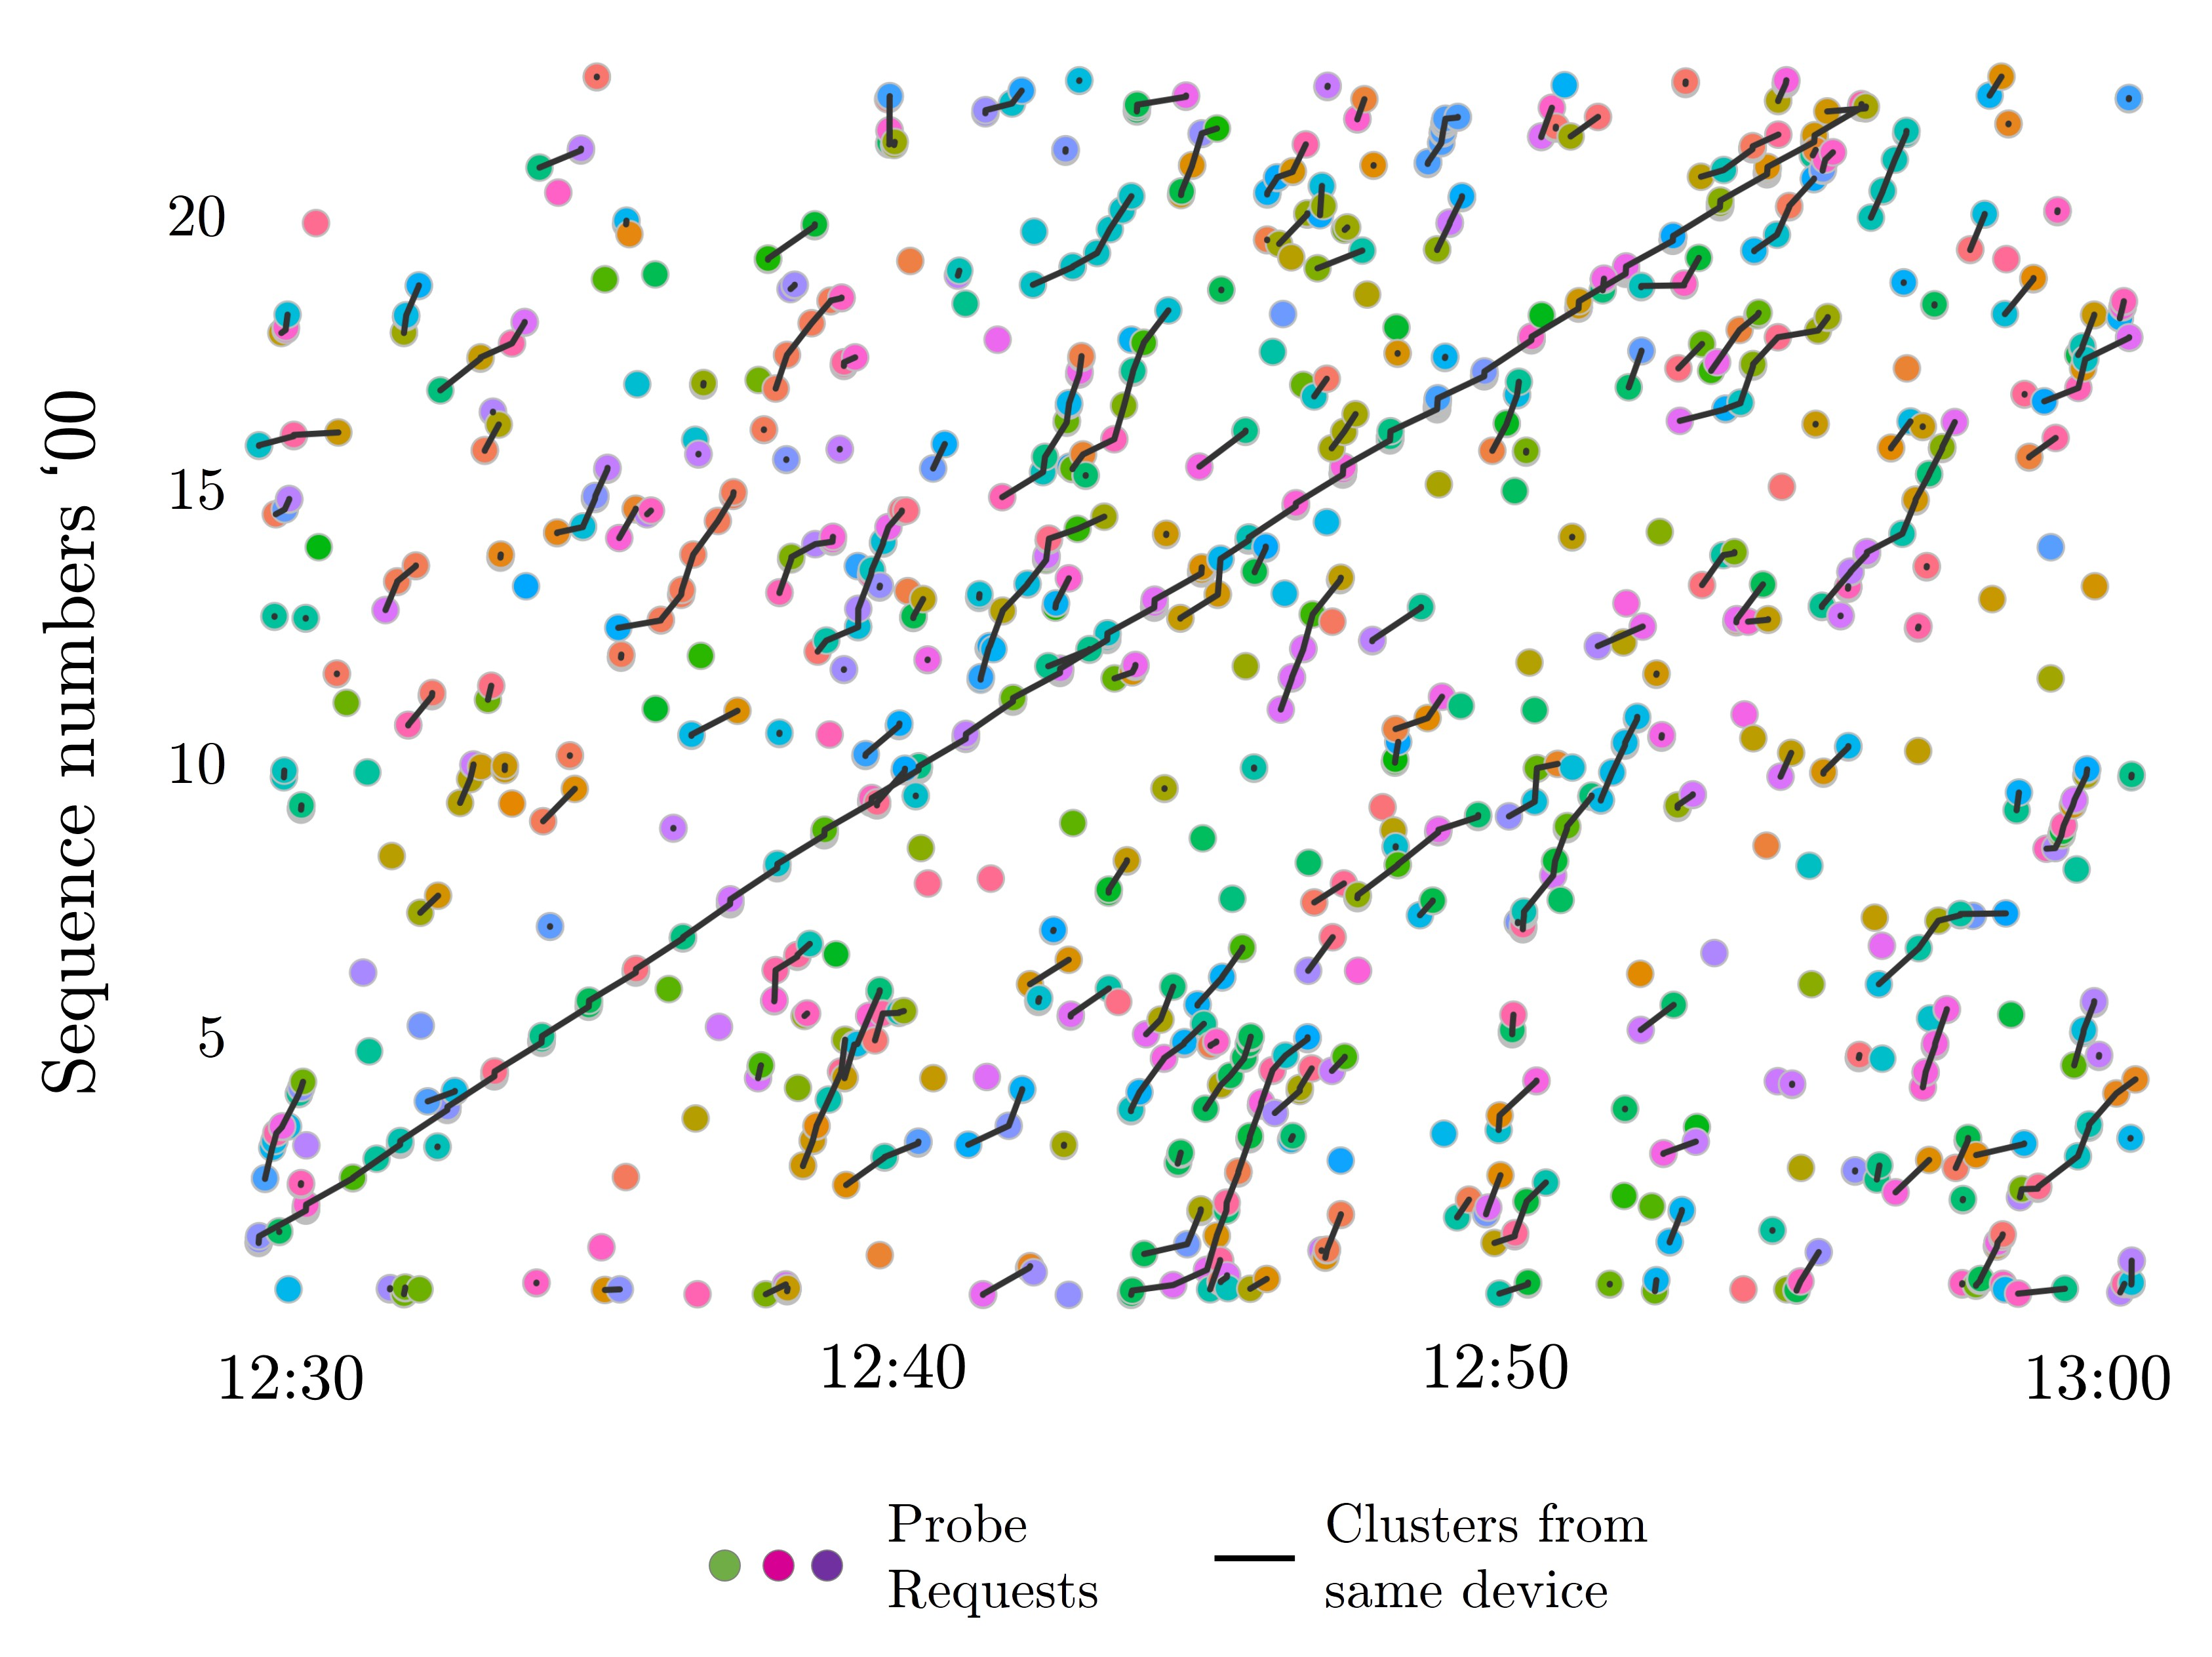
\includegraphics [width=\linewidth] {images/pilot_clustering.jpeg}
		\caption{Clustering probe requests based on increasing sequence numbers present in them. The dots are individual probe requests and the red lines connect probe requests within the same cluster which are generated by the same mobile device.}
		\label{pilot_clustering}
	\end{center}
\end{figure}

The minute by minute comparision of counts from the filtering processes along with the ground truth is shown in Figure \ref{pilot_comparison} From the pilot study, we find that both classification and clustering methods work on complex real world data and results in a final pedestrian counts within a error of 20\%.
We also find `k-means' and `quantile' are best algorithms for classifying signal strengths.

\begin{figure}
	\begin{center}
		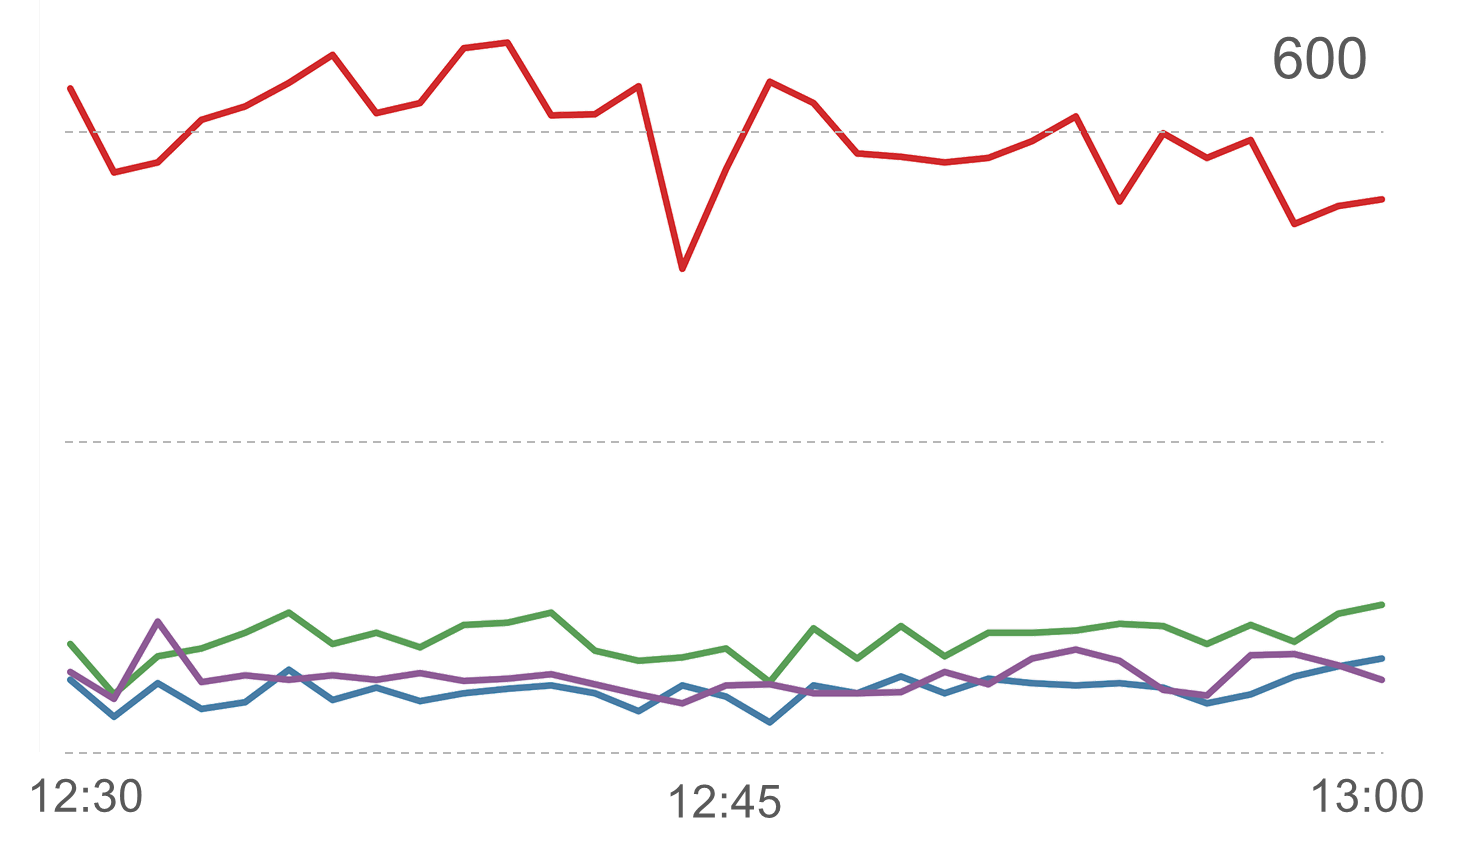
\includegraphics [width=0.85\linewidth] {images/pilot_counts_comparision.png}
		\caption{Comparision of counts after filtering with manual counts}
		\label{pilot_comparison}
	\end{center}
\end{figure}


